\documentclass[man]{apa6}
\usepackage{lmodern}
\usepackage{amssymb,amsmath}
\usepackage{ifxetex,ifluatex}
\usepackage{fixltx2e} % provides \textsubscript
\ifnum 0\ifxetex 1\fi\ifluatex 1\fi=0 % if pdftex
  \usepackage[T1]{fontenc}
  \usepackage[utf8]{inputenc}
\else % if luatex or xelatex
  \ifxetex
    \usepackage{mathspec}
  \else
    \usepackage{fontspec}
  \fi
  \defaultfontfeatures{Ligatures=TeX,Scale=MatchLowercase}
\fi
% use upquote if available, for straight quotes in verbatim environments
\IfFileExists{upquote.sty}{\usepackage{upquote}}{}
% use microtype if available
\IfFileExists{microtype.sty}{%
\usepackage{microtype}
\UseMicrotypeSet[protrusion]{basicmath} % disable protrusion for tt fonts
}{}
\usepackage{hyperref}
\hypersetup{unicode=true,
            pdftitle={Animal Tracking with TRAJR},
            pdfauthor={Richard Troise},
            pdfkeywords={keywords},
            pdfborder={0 0 0},
            breaklinks=true}
\urlstyle{same}  % don't use monospace font for urls
\usepackage{graphicx,grffile}
\makeatletter
\def\maxwidth{\ifdim\Gin@nat@width>\linewidth\linewidth\else\Gin@nat@width\fi}
\def\maxheight{\ifdim\Gin@nat@height>\textheight\textheight\else\Gin@nat@height\fi}
\makeatother
% Scale images if necessary, so that they will not overflow the page
% margins by default, and it is still possible to overwrite the defaults
% using explicit options in \includegraphics[width, height, ...]{}
\setkeys{Gin}{width=\maxwidth,height=\maxheight,keepaspectratio}
\IfFileExists{parskip.sty}{%
\usepackage{parskip}
}{% else
\setlength{\parindent}{0pt}
\setlength{\parskip}{6pt plus 2pt minus 1pt}
}
\setlength{\emergencystretch}{3em}  % prevent overfull lines
\providecommand{\tightlist}{%
  \setlength{\itemsep}{0pt}\setlength{\parskip}{0pt}}
\setcounter{secnumdepth}{0}
% Redefines (sub)paragraphs to behave more like sections
\ifx\paragraph\undefined\else
\let\oldparagraph\paragraph
\renewcommand{\paragraph}[1]{\oldparagraph{#1}\mbox{}}
\fi
\ifx\subparagraph\undefined\else
\let\oldsubparagraph\subparagraph
\renewcommand{\subparagraph}[1]{\oldsubparagraph{#1}\mbox{}}
\fi

%%% Use protect on footnotes to avoid problems with footnotes in titles
\let\rmarkdownfootnote\footnote%
\def\footnote{\protect\rmarkdownfootnote}


  \title{Animal Tracking with TRAJR}
    \author{Richard Troise\textsuperscript{1}}
    \date{}
  
\shorttitle{Animal Tracking with TRAJR}
\affiliation{
\vspace{0.5cm}
\textsuperscript{1} Brooklyn College}
\keywords{keywords\newline\indent Word count: X}
\usepackage{csquotes}
\usepackage{upgreek}
\captionsetup{font=singlespacing,justification=justified}

\usepackage{longtable}
\usepackage{lscape}
\usepackage{multirow}
\usepackage{tabularx}
\usepackage[flushleft]{threeparttable}
\usepackage{threeparttablex}

\newenvironment{lltable}{\begin{landscape}\begin{center}\begin{ThreePartTable}}{\end{ThreePartTable}\end{center}\end{landscape}}

\makeatletter
\newcommand\LastLTentrywidth{1em}
\newlength\longtablewidth
\setlength{\longtablewidth}{1in}
\newcommand{\getlongtablewidth}{\begingroup \ifcsname LT@\roman{LT@tables}\endcsname \global\longtablewidth=0pt \renewcommand{\LT@entry}[2]{\global\advance\longtablewidth by ##2\relax\gdef\LastLTentrywidth{##2}}\@nameuse{LT@\roman{LT@tables}} \fi \endgroup}


\DeclareDelayedFloatFlavor{ThreePartTable}{table}
\DeclareDelayedFloatFlavor{lltable}{table}
\DeclareDelayedFloatFlavor*{longtable}{table}
\makeatletter
\renewcommand{\efloat@iwrite}[1]{\immediate\expandafter\protected@write\csname efloat@post#1\endcsname{}}
\makeatother

\authornote{Add complete departmental affiliations for each
author here. Each new line herein must be indented, like this line.

Enter author note here.

Correspondence concerning this article should be addressed to Richard
Troise, Postal address. E-mail:
\href{mailto:my@email.com}{\nolinkurl{my@email.com}}}

\abstract{
A compact demonstration on the R-package TRAJR, shows that any set of
Cartesian coordinates can be transformed into a trajectory object and
information can be collected on that object. One example borrowed from
the package tutorial, was on how to calculate average velocity,
sinuosity, and the Emax value (straightness) along the whole trajectory
path. This demonstration shows how two different trajectories, one with
seemingly more curvature, displays different values of sinuosity and
straightness. Though more examples could reflect the depth of
applications, one could implement such tools in animal learning
experiments.


}

\begin{document}
\maketitle

The R-package \enquote{Trajr} had been recently implemented for
biological research with the idea of tracking moving animals.
Psychologists could make use of trajectories in animal learning studies,
specifically when the animals utilize path integration. The tracking of
an animal can first be recorded via video footage or GPS tracking. The
data can then be imported in R, where it is transformed into a
\enquote{trajectory} object. The object itself contains: the trajectory
data (as a data frame of coordinates and time steps), the time steps
converted into a numerical unit, displacement information, and the polar
coordinate-equivalent from Cartesian. From there, any user can choose to
plot the trajectory and perform various calculations. The function
\enquote{TrajDistance} for examples, determines the shortest distance
travelled based on the start and end point of a path. The demonstration
utilizes a custom function, built by the original author of Trajr McLean
and Volponi (2018), to show what the general output looks like when
calculating the variables \enquote{average speed}, \enquote{sinuosity},
and \enquote{straightness}. The speed is simply calculated as position
over time. Sinuosity can be thought as how much curvature contributes to
the total path relative to a shortest line connecting the two
\enquote{start} and \enquote{end} points. The greater the number, the
more bending of the path there is. The index of straightness is inferred
by an \enquote{Emax} value. Straighter paths hold higher values, and the
range is allowed to approach infinity.

\section{Methods}\label{methods}

\subsection{Participants}\label{participants}

No participants were used in this demonstration.

\subsection{Material}\label{material}

\begin{verbatim}
## Warning: package 'trajr' was built under R version 3.5.3
\end{verbatim}

\begin{verbatim}
## Warning: package 'xtable' was built under R version 3.5.3
\end{verbatim}

\begin{figure}
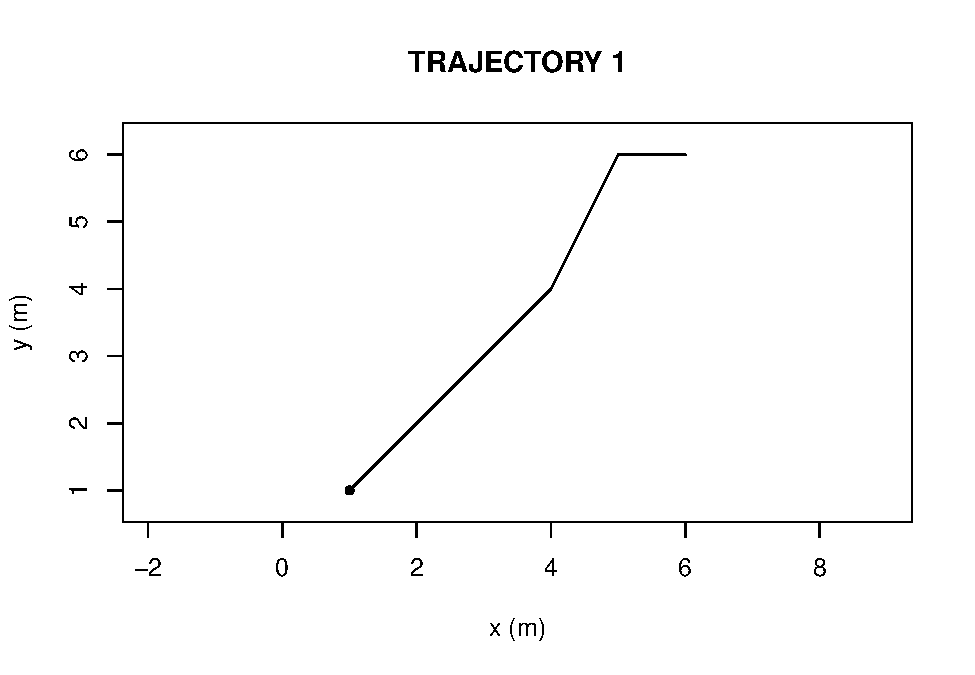
\includegraphics[height=300px]{final_paper_files/figure-latex/unnamed-chunk-1-1} \caption{ }\label{fig:unnamed-chunk-1}
\end{figure}

\begin{figure}
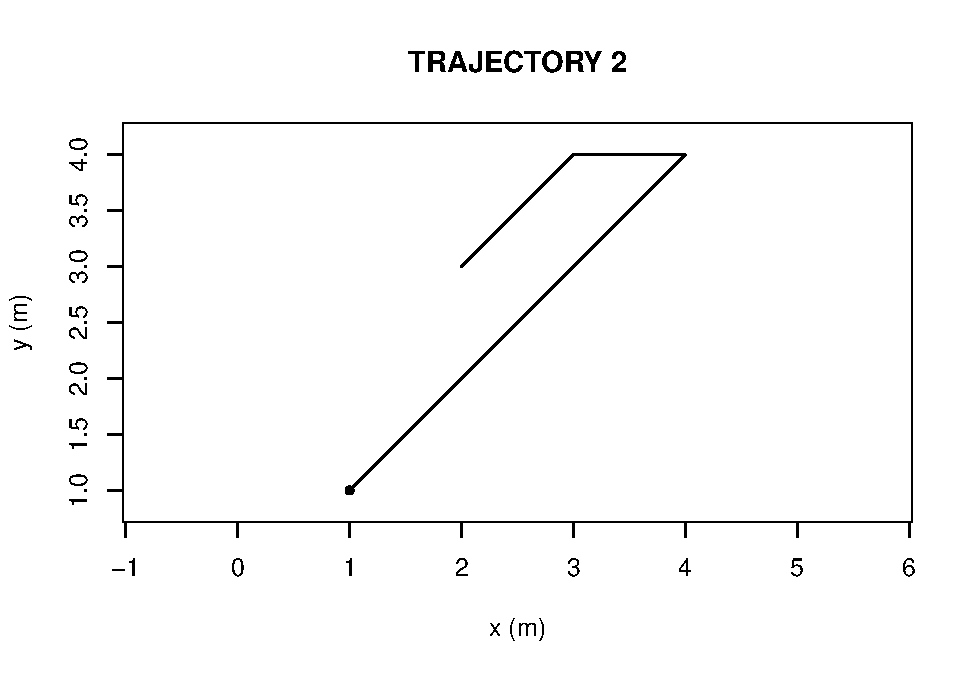
\includegraphics[height=300px]{final_paper_files/figure-latex/unnamed-chunk-2-1} \caption{ }\label{fig:unnamed-chunk-2}
\end{figure}

\subsection{Procedure}\label{procedure}

We first compiled two hypothetical trajectories in R-studio, a data
frame with a set of six x-coordinates (in units of meters),
y-coordinates, and time steps (unitless). The \enquote{TrajFromCoords}
function, allows for the conversion of a data frame into a trajectory
object. We then plotted the two objects to visualize the paths.

The function \enquote{characteriseTrajectory} takes a single trajectory
object and computes the average speed and standard deviation (that some
animal would take) based on the derivatives calculated via
\enquote{TrajDerivatives}. \enquote{TrajSinuosity} and
\enquote{TrajEmax} are the functions that compute the sinuosity and
straightness of the two paths. Lastly, the chracterizing function stores
the computed information in the list which can be displayed at once or
individually.

\subsection{Data analysis}\label{data-analysis}

We used R (Version 3.5.0; R Core Team, 2018) and the R-packages
\emph{papaja} (Version 0.1.0.9842; Aust \& Barth, 2018), and
\emph{xtable} (Version 1.8.4; Dahl, Scott, Roosen, Magnusson, \&
Swinton, 2019) for all our analyses.

\section{Results}\label{results}

The sinuosity and E-max values were greater in Trajectory 2 than
Trajectory 1.

\begin{tabular}{r|l}
\hline
Trajectory1 & Parameter\\
\hline
74.7870866 & Avg.Speed\\
\hline
22.5524852 & Std.Speed\\
\hline
0.6038492 & Sinuosity\\
\hline
5.6213862 & Emax\\
\hline
\end{tabular}

\begin{tabular}{r|l}
\hline
Trajectory2 & Parameter\\
\hline
66.568543 & Avg.Speed\\
\hline
9.262097 & Std.Speed\\
\hline
1.135893 & Sinuosity\\
\hline
1.000000 & Emax\\
\hline
\end{tabular}

\section{Discussion}\label{discussion}

Based on the outputs of the \enquote{characteriseTrajectory}, The first
and second trajectories (Figure 1 and Figure 2) differ in their
sinuosity and Emax due to the nature of the paths themselves. The
bending behavior, is what causes the second trajectory, in Figure 2
(Appendix) to possess a higher turning value(sinuosity) and lower Emax
(straightness) than in the first trajectory, in Figure 1.

\newpage

\section{References}\label{references}

\begin{verbatim}
## Warning in readLines(file): incomplete final line found on 'r-
## references.bib'
\end{verbatim}

\begingroup
\setlength{\parindent}{-0.5in} \setlength{\leftskip}{0.5in}

\hypertarget{refs}{}
\hypertarget{ref-R-papaja}{}
Aust, F., \& Barth, M. (2018). \emph{papaja: Create APA manuscripts with
R Markdown}. Retrieved from \url{https://github.com/crsh/papaja}

\hypertarget{ref-R-xtable}{}
Dahl, D. B., Scott, D., Roosen, C., Magnusson, A., \& Swinton, J.
(2019). \emph{Xtable: Export tables to latex or html}. Retrieved from
\url{https://CRAN.R-project.org/package=xtable}

\hypertarget{ref-Mclean2018}{}
McLean, D. J., \& Volponi, M. A. S. (2018). Trajr: An r package for
characterisation of animal trajectories. \emph{Ethology}, \emph{124}(6).
doi:\href{https://doi.org/10.1111/eth.12739}{10.1111/eth.12739}

\hypertarget{ref-R-base}{}
R Core Team. (2018). \emph{R: A language and environment for statistical
computing}. Vienna, Austria: R Foundation for Statistical Computing.
Retrieved from \url{https://www.R-project.org/}

\endgroup


\end{document}
